\documentclass[12pt]{article}
\usepackage[a4paper, margin=.30in]{geometry}
\usepackage{graphicx ,
            wrapfig,
            xcolor, 
            enumerate,
            amsmath,fontenc
            }

\newcommand\headerMe[2]{\noindent{}#1\hfill#2}
\renewcommand{\thesection}{\Roman{section}}

\title{Leçon N 6 : Le mouvement}
\author{Zakaria HAOUZAN}
\date{\today}

\begin{document}
% headers --------------
\headerMe{Matière : Physique-Chimie}{Professeur : Zakaria HAOUZAN}\\
\headerMe{Unité : La Mécanique}{Établissement : Lycée SKHOR qualifiant}\\
\headerMe{Niveau : TCS}{Heure : 6H}\\

% ------Content ________
\begin{center}

    \Large{Leçon $N^{\circ}6$: \color{red}Le Mouvement}
\end{center}

\section{\color{red}Relativité du mouvement:}
\subsection{\color{green}Mise en évidence}
Dans l'exemple suivant on peut donner plusieurs descriptions au mouvement de l'observateur B.\\
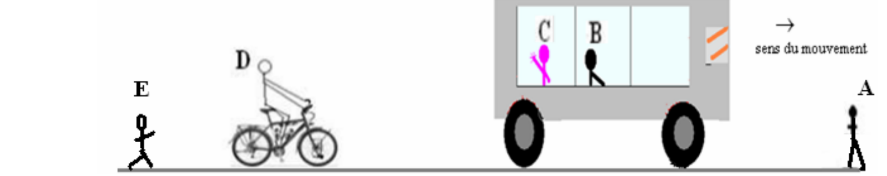
\includegraphics[width=0.75\textwidth]{./img/img00.png}\\
B est immobile par rapport à C.\\
B s'éloigne par rapport à D et il s'éloigne encore plus vite par rapport à E.\\
B s'approche par rapport à A.\\
Ce sont des descriptions différentes pour le même mouvement ce qui montre que l'étude du mouvement d'un
corps est relatif il dépend du référentiel choisi d’où la relativité du mouvement .


\subsection{Conclusion}
Le mouvement est relatif au référentiel choisi, c'est à dire que les corps ne se déplacent que par rapport à
d'autres corps.\\
Donc pour étudier le mouvement d'un corps on doit choisir un référentiel fixe puis un repère d'espace et un
repère de temps liés à ce référentiel.

\subsection{Repère d'espace}
Pour repérer la position du mobile dans le référentiel choisi on utilise un repère d'espace.\\
\underline{$1^{er}$ cas : Si le mouvement est rectiligne} (mouvement d'un train par exemple.)\\
Dans ce cas le repère d'espace est un axe $(O, \vec{i})$ orienté dans le sens du mouvement . $\overrightarrow{OM} = x\vec{i}$

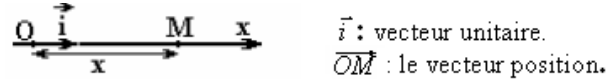
\includegraphics[width=0.4\textwidth]{./img/img01.png}
\\
\begin{wrapfigure}{r}{0.3\textwidth}
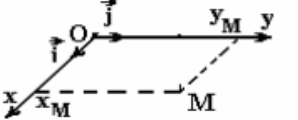
\includegraphics[width=0.3\textwidth]{./img/img02.png}
\end{wrapfigure}
\underline{$2^{\grave{e}me}$ cas : Si le mouvement est plan} ( mouvement d'une fourmi par ex. sur la table.)

Dans ce cas le repère d'espace est un repère orthonormé $(O, \vec{i}, \vec{j})$ confondu avec le plan du mouvement.
\\Le vecteur position $\overrightarrow{OM} = x.\vec{i} + y.\vec{j}$ avec son Module : $OM =\sqrt{x^2 + y^2} $



\underline{$3^{\grave{e}me}$ cas : Si le mouvement est spatial: }( mouvement d'une abeille dans l'espace par ex.)
\\Dans ce cas le repère d'espace est un repère orthonormé direct $(O, \vec{i}, \vec{j}, \vec{k})$. 
\\Le vecteur position $\overrightarrow{OM} = x.\vec{i} + y.\vec{j} + z.\vec{k}$ avec son Module : $OM =\sqrt{x^2 + y^2 + z^2} $.
\\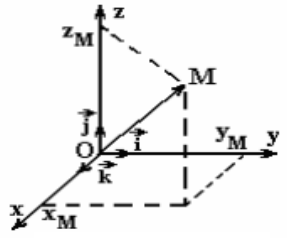
\includegraphics[width=0.2\textwidth]{./img/img03.png}

\subsection{Repère de temps : }
Aucours de son mouvement le mobile occupe des différentes positions et ses coordonnées varient en fonction du
temps .

Pour déterminer la position du mobile à un instant donné on doit choisir une origine de temps qui correspond à
la position du mobile à l'instant t=0.(c'est ce qu'on appelle repère de temps)
L'unité de mesure du temps dans le système d'unités international est la seconde (s).
On donne quelques multiples et sous multiples de la seconde :

\begin{tabular}{|c|c|c|}
    \hline
    nom             & symbole       & La valeur\\\hline
    microseconde    & $\mu.s$    & $1.\mu.s = 10^{-6}s$\\\hline
    milliseconde    & $m.s$         & $1.m.s = 10^{-3}s$\\\hline
    minute          & $min$         & $1.min = 60s$\\\hline
    heure           & $h$           & $1.h = 60min = 3600s$\\\hline
    jour            & $j$           & $1.j = 24h$\\\hline
    L'année         & $an$          & $1.an = 365j$\\\hline

\end{tabular}


\subsection{La trajectoire}
La trajectoire est l'ensemble des positions successives occupées par le mobile au cours de son mouvement.(elle
peut être rectiligne , curviligne ou bien circulaire....).
\\$$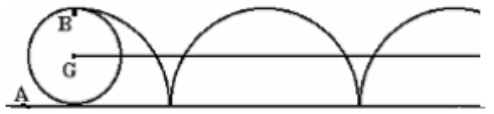
\includegraphics[width=0.4\textwidth]{./img/img04.png}$$


%______________sub___Section 2_______________________________
\subsection{La Vitesse : }
\subsection{La vitesse moyenne : }
\subsubsection{Définition : }
La vitesse moyenne d'un mobile est égale au quotient de la distance d parcourue par la durée t du parcours .
$$v = \frac{d}{t}$$
$$d : la\; distance \; parcourus \;(m),\hspace{1cm} t:\; dur\acute{e}e \;du parcours(s),\hspace{1cm}v : \;vitesse\; moyenne \;(m/s)$$

\subsubsection{Exercice d'application : }
Un train TGV parcourt une distance d = 450 kmen 1h23min20s.\\
1-Calculer sa vitesse moyenne en (m/s) puis en (km/s).\\
2-Le même train précédent parcourt une distance d'=630 km .Quelle est la durée de parcours? 

\subsection{La Vitesse instantanée : }
\subsubsection{Définition : }
\begin{wrapfigure}{r}{0.2\textwidth}
    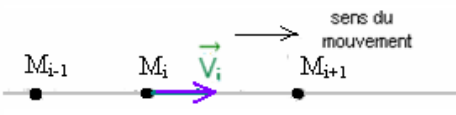
\includegraphics[width=0.2\textwidth]{./img/img05.png}
\end{wrapfigure}

La vitesse instantanée d'un mobile est sa vitesse $\grave{a}$ un instant donnée.
\\Apartir  d'un enregistrement, on calcul la valeur de la vitesse instantanée du mobile au point $M_i$ par la méthode d'encadrement suivant : $$v_i = \frac{M_{i-1}M_{i+1}}{t_{i+1}-t_{i-1}}$$
Le temps qui sépare deux points successifs de l'enregistrement est égale $\grave{a}\; \tau $ donc :$ 2\tau = t_{i+1}-t_{i-1}$ 
$$v_i = \frac{M_{i-1}M_{i+1}}{2\tau}$$

\begin{wrapfigure}[4]{r}{0.4\textwidth}
    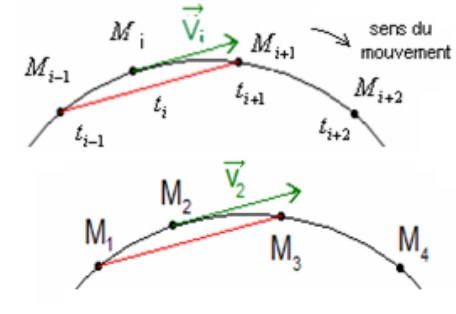
\includegraphics[width=0.4\textwidth]{./img/img07.png}
\end{wrapfigure}

\underline{Le vecteur vitesse instantanée $\vec{v_i}$  est caractérisé par :}\\
origine : position $M_i$ du point mobile $\grave{a}$ l'instant $t_i$.\\
direction : tangent $\grave{a}$ la trajectoire en ce point . \\
sens  : celui du mouvement .\\
norme : $v_i = \frac{M_{i-1}M_{i+1}}{2\tau}$ en m/s


Exemples : 
\\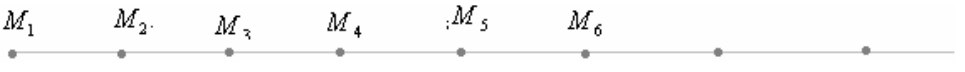
\includegraphics[width=0.5\textwidth]{./img/img06.png}
\\donc :  $v_2 = \frac{M_1M_3}{2\tau}$, $v_3 = \frac{M_2M_4}{2\tau}$, $v_4 = \frac{M_3M_5}{2\tau}$
\\\underline{Remarque : Si la trajectoire est circulaire , l'arc : $\widehat{M_{i-1}M_{i+1}} \approx M_{i-1}M_{i+1}$}
\\Exemple : la vitesse instantanée au point $M_2$ est : $v_2 = \frac{M_1M_3}{2\tau}$

\subsection{Exercice d'application : }
\begin{wrapfigure}[4]{r}{0.4\textwidth}
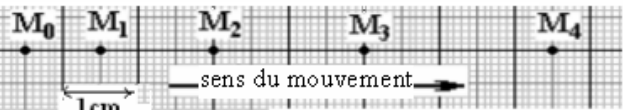
\includegraphics[width=0.4\textwidth]{./img/img08.png}
\end{wrapfigure}
On donne l'enregistrement du mouvement d'un autoporteur sur une table horizontale :
L'intervalle de temps qui sépare deux enregistrement successifs est $\tau = 50ms$.
\\1-Calculer la vitesse instantanée aux points M1 puis M2 puis au point M3.
\\2-Représentez le vecteur vitesse au point M3 $\grave{a}$ l'échelle suivant 1cm $\rightarrow$ $0.3m.s^{-1}$



%%%%%%%%%%%%%%%%%%%%%%_______________________Section __________II________________

\section{Le mouvement rectiligne uniforme : }
\subsection{Mouvement rectiligne : }
Un mouvement est dit rectiligne s'il s'effectue selon une trajectoire qui est une droite.
\subsection{Mouvement rectiligne uniforme : }
Le Mouvement rectiligne est dit uniforme si son vecteur vitesse est constant en valeur, en direction et en sens $\vec{v} = \overrightarrow{constante}$
\subsection{Equation horaire d'un mouvement rectiligne uniforme : }
La vitesse v d'un mobile en mouvement rectiligne uniforme est constante et l'équation horaire de son mouvement x = f(t) est une fonction affine de temps de forme : $x = v.t + x_0$ \\x : abscisse du mobile à l'instant t en (m).\\
v : valeur valeur algébrique de la vitesse du mobile en (m/s)
\\$x_0$ : l'abscisse du mobile à l'instant t = 0 en (m).
\\
Remarque  :Si le mobile se déplace dans le même sens que l'axe ox, $v>0$. Si le mobile se déplace dans le sens contraire que l'axe ox, $v<0$.

\subsection{Exercice d'application : }
Aucours du mouvement rectiligne uniforme d'un autoporteur (S) on a obtenu l'enregistrement suivant Durant lequel l'intervalle de temps qui sépare deux points successifs est $\tau = 40ms$.
\begin{center}
\centering
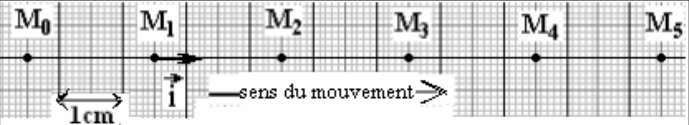
\includegraphics[width=0.5\textwidth]{./img/img09.png}
\end{center}
1- Quelle est la nature du mouvement de (S)?
\\2- Déterminer la valeur de la vitesse de S
\\3- Completez le remplissage du tableau suivant sachant qu'à l'instant t = 0 le mobile passe par le point $M_2$.
\begin{center}
\begin{tabular}{|c|c|c|c|c|}
    \hline
    position        & $M_2$ & $M_3$ & $M_4$ &$M_5$     \\\hline
    x(cm)           &       &          & &\\\hline
    t(s)            &       &          & &\\\hline

\end{tabular}
\end{center}
\section{Le Mouvement circulaire uniforme : }
\subsection{Définition :}
Un mobile M est en mouvement circulaire uniforme si sa trajectoire est un cercle (ou un arc de cercle) et sa vitesse est constante en norme aucours du temps.c'est a dire que dans ce cas le vecteur vitesse ne garde pas la même direction et le même sens.
\begin{center}
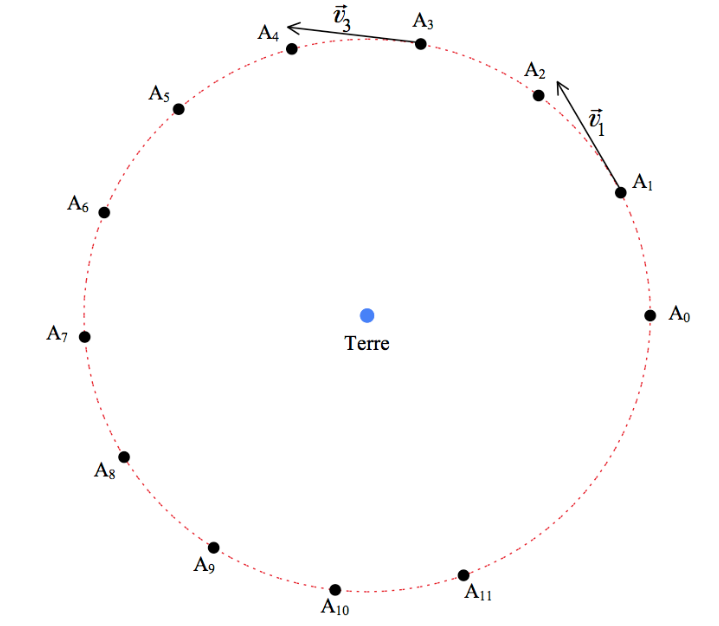
\includegraphics[width=0.4\textwidth]{./img/img10.png}
\end{center}

\subsection{La période et la fréquence : }
La période d'un mouvement de rotation circulaire uniforme est la durée d'un tour : $$T = \frac{2.\pi.R}{V}$$ avec V : la vitesse en (m/s) et R : le rayon en (m)
\\la fréquence f est égale $\grave{a}$ l'inverse de la période : $$f = \frac{1}{T}$$
la fréquence s'exprime en Hertz (Hz).



\end{document}
